\section{Theory}
\label{sec:theory}




\subsection{How to control covariance}

For controlling covariance, we can use friction. When the swarm move across the wall, friction force will apply to the robots that are going across the wall, and so they will have less velocity than the free ones. With this difference we have broken the symmetry and can control the covariance. As we can see from Eq. ~\ref{eq:frictioneqn}, total force for going forward will change. 

\begin{align}
\label{eq:frictioneqn}
F_f &= \mu_f N \nonumber\\
N &= F cos\theta \nonumber\\
F_{forward} &= F sin\theta - F_f
\end{align}
where $F$ is our control input. As shown in Fig. ~\ref{fig:friction}, the total force for going forward is less than a free robot. So we can reduce speed of some robots with friction.

\begin{figure}[h]
\begin{center}
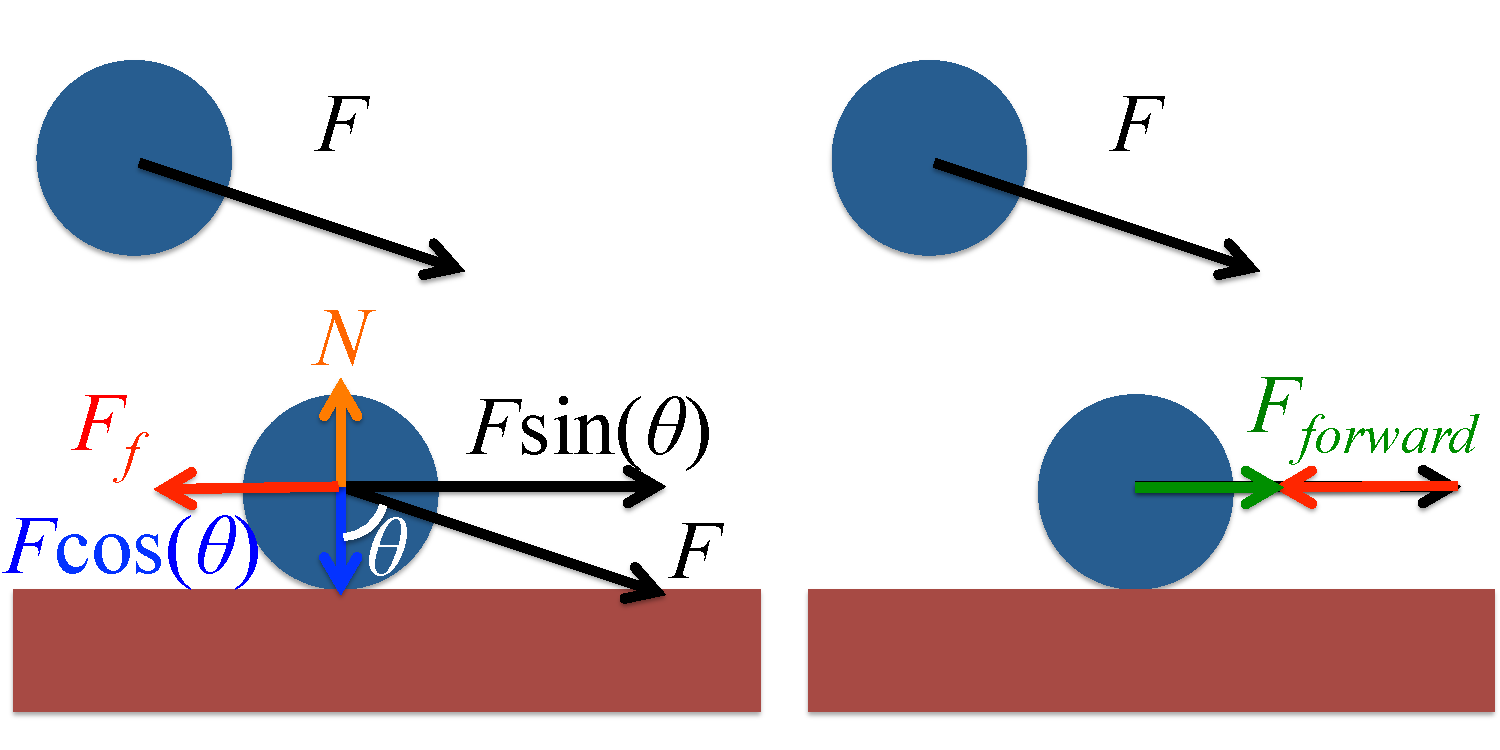
\includegraphics[width=\columnwidth]{friction.png}
\caption{When the robot is near the wall, the overall force for going forward is less than a free robot because of the friction.}
\label{fig:friction}
\end{center}
\end{figure} 


